\chapter{Conclusions and Future Work}

\section{Conclusions}

Given the deluge of spectroscopic data from modern surveys, manual methods, rule-based methods and certain machine-learning methods may not be suitable to address the twin problems of identification and classification of non-typical spectra such as H$\alpha$ emission-line stars. The preceding chapters demonstrated that these challenges can be overcome using a combination of dimensionality reduction, anomaly detection and spectral-morphology-based clustering that utilises dynamic time warping and agglomerative hierarchical clustering. 

The methods presented in this work provide significant advantages over other recent methods that rely on manual human intervention to identify and classify P Cygni, inverse P Cygni and other species of emission-line spectra such as \citet{zhang2021catalog} and \citet{zhao2012lamost}. In addition to requiring minimal human intervention when setting the machine learning parameters, a key advantage is that these methods do not require a labelled training data set, thus further reducing the need for human intervention.  This work demonstrated that if the code, data structures, algorithms and strategy are picked carefully, emission-line spectra can be identified and classified with reasonable computational efficiency with complexity $O(N)$, without requiring a human being to review manually thousands, hundreds of thousands  or even potentially millions of spectra.

The autoencoder used in this analysis functions as an anomaly detector, capable of flagging spectra with emission-line features. This is a mature and well established methodology in domains such as credit card fraud detection, and the approach can be extended to other areas of astronomy that require the detection of atypical signals from a large volume of more typical signals. Similarly, dynamic time warping is a well-established signal processing and machine-learning method that is sensitive to shapes and morphologies of signals over other features, and consequently can be applied to other fields in astronomy where the morphological features of a signal play a dominant role over other considerations. To this author's knowledge, casting spectra as time series and using DTW has not been used to identify and classify astronomical spectra in the literature, and consequently is a novel approach. 

With agglomerative hierarchical clustering, this work demonstrated that the number of clusters and consequently the depth of the hierarchical tree is sensitive to the population mix over which the algorithm is run. In the case of GALAH DR3, the maximum numbers of P Cygni and inverse P Cygni spectra were separated out when the number of clusters was set to 45. While the literature that informed this work suggested that the number of clusters must be greater than 6 and under 10, determining this value for the emission-line population present in DR3 required an iterative approach of setting the number of clusters and tracking the number of spectra separated from the primary population as P Cygni and inverse P Cygni. While this is not particularly time consuming, it does require human intervention to define and specify a parameter to extract meaningful and useful clusters from the broader emission-line population. 

The resulting larger number of clusters was useful for the classification of more atypical and exotic spectra. This "over-classification" could be extremely beneficial for researchers who study still more exotic emission-line phenomena, as well as being a useful mechanism to foster further analysis on whether some of the minority classes can indeed be combined with the majority classes that appear at higher levels of the hierarchical tree. Such decisions can be left to the researcher on the basis of what specific type of object is being studied. For example, it is clear that the clusters presented below can be combined meaningfully into a single P Cygni cluster, thus netting a total of 296 P Cygni spectra from the DR3 sample. Over-classification, prior to merging, is thus a beneficial outcome of this approach. 

The methodology discussed in Chapter 6 is sensitive to a number of factors, including, the type and population of stars captured by a survey has a direct impact on the performance of this method. For example, if a survey is biased towards young stars or, as in the case of the Gaia ESO survey, open clusters, it is reasonable to expect a high proportion of emission-line stars in the raw data. In this scenario the researcher may have to adjust or remove the anomaly detection-based autoencoder from the pipeline suggested in Chapter 6. Autoencoders can excel at detecting anomalies in more typical-looking data, but if the data contain a majority of atypical spectra, the performance of the autoencoder must be evaluated more thoroughly; this work hypothesises that in such scenarios the performance may degrade and hence it may be beneficial to bypass or remove this step and proceed directly to computing DTW distances, followed by agglomerative hierarchical clustering. 
%The results from the autoencoder are also sensitive to the equivalent width cut-off criterion described in Chapter 6. Čotar et al. placed this value at 0.25, and the effect of this cut-off on the number of emission-line spectra that can be automatically identified would have to be modeled. This was beyond the scope of this present work. Similar to the number of clusters, it can be hypothesised that this value is population-dependent, but perhaps more constrained than the number of clusters. 

The equivalent width cut-off that selects H$\alpha$ emission-line spectra from the broader DR3 data set is another significant parameter that impacts the final population of classified emission-line stars. \citet{vcotar2021galah} placed this value at 0.25, but the degree to which this parameter should be tailored to the underlying sample population remains unclear; unlike the number of clusters, there exists no suitable guiding values for this parameter in the literature apart from the figure presented in \citet{vcotar2021galah}. This parameter may be linked to the decoding accuracy of the autoencoder, but exploring the details of this relationship would be beyond the scope of this work.

It is clear that dimensionality reduction techniques such as t-SNE and autoencoders must thus be used judiciously based on the type of population being surveyed. While t-SNE is widely considered to be a general purpose method, it has proven less effective at identifying and classifying emission-line stars than the combined application of an autoencoder, followed by dynamic time warping and agglomerative clustering. 

\begin{figure}[!htb]
\centering
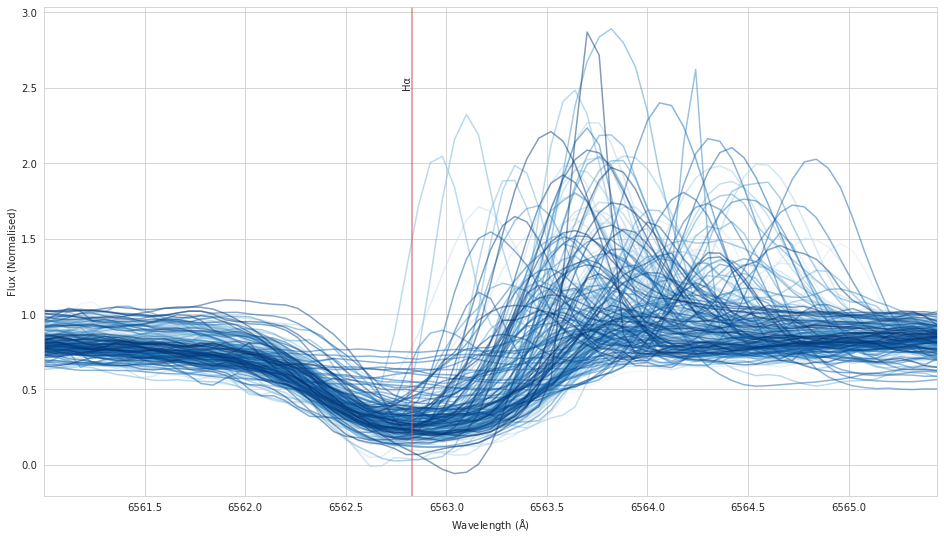
\includegraphics[scale=0.45]{figures/p cygni ensemble.png}
\caption{Ensemble plot of 243 P Cygni spectra identified in GALAH DR3 using DTW.}
\end{figure}

\begin{figure}[!htb]
\centering
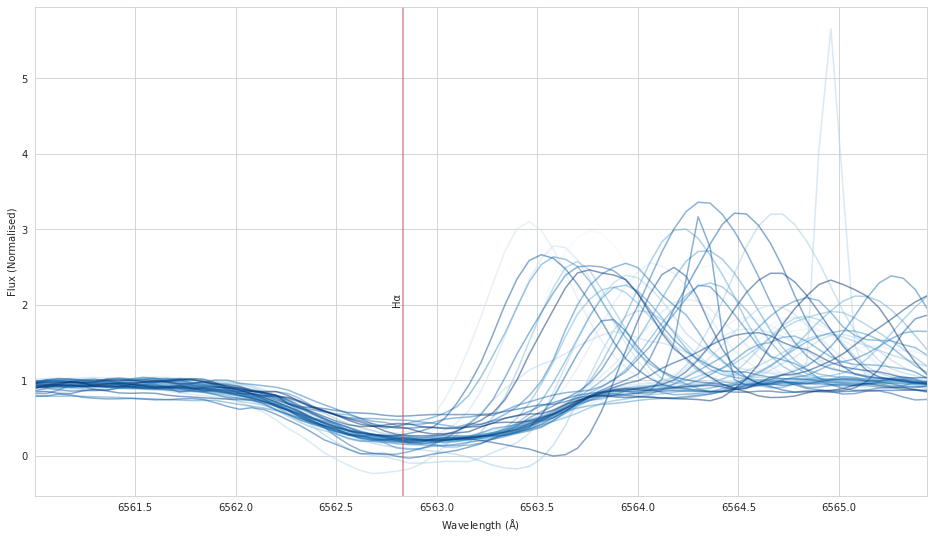
\includegraphics[scale=0.45]{figures/p cugni 2.png}
\caption{Ensemble plot of 53 P Cygni spectra identified in GALAH DR3 using DTW. These were not included in the main P Cygni cluster but rather appeared in a separate group, likely due to a less prominent absorption feature to the blueward of H$\alpha$. Hence, these can be combined with the majority P Cygni cluster to give 296 P Cygni spectra in total.}
\end{figure}


\section{Future Work and Potential Applications of the Methods Discussed in This Work}

This section presents several future directions and starting points that go beyond this work. Based on the results in Chapter 6, this work can be extended to identify and classify emission-line spectra in future releases of GALAH as well as surveys such as Gaia. This work also prompts further exploration of dimensionality reduction methods that are suited for the exploration of spectra from large-scale surveys. 

\subsection{Emission-line Spectra in GALAH DR4}

The GALAH survey has yielded significantly more data since DR3, with over 800,000 unique targets observed to date. While this has not yet been released to the public, they are available within the GALAH collaboration, and hence can be run through the pipeline described in this work. Once the emission-line spectra in this larger sample have been identified and classified, a catalogue of emission-line stars, and in particular P Cygni and inverse P Cygni spectra can be produced, and ideally published, including cross-matches with Gaia and literature (e.g., via SIMBAD). Furthermore, a detailed analysis of this larger sample would provide an opportunity to—as mentioned in the previous section—modelling the sensitivity of the equivalent width cut-off and explore the impact of the number of clusters on classification accuracy.

\subsection{Characterising Emission-line Spectra}

Given the large number of classes, and the 296 P Cygni and 219 inverse P Cygni spectra that were identified, it would be extremely useful to characterise each group based on the type of star producing those spectra. Crucially, the stellar parameters of these members will also warrant reevaluation, as the spectra deviate significantly from more typical spectra, and so the stellar parameters for these objects determined by standard pipelines are likely to have higher uncertainties compared to those of more typical spectra. Parameters such as effective temperature and stellar masses can be reevaluated for these emission-line spectra outside the primary pipelines. For the various categories of emission-line stars, it would be useful to measure  the properties of their emission spectra, for example the inflow and outflow wind velocities of P Cygni and inverse P Cygni spectra. Expanding the binary mask that was applied to isolate the region near the H$\alpha$ region could also potentially reveal objects that have high wind velocities. The methods presented in this work can be suitably adapted to study these high wind velocity objects.

\subsection{Extension to Other Domains in Astronomy}

Dynamic time (wavelength) warping and agglomerative hierarchical clustering are sufficiently generalised methods that can be adapted to a range of problems and subdomains: for example, they can be used to cluster light curves, gravitational wave signals and radio spectra. These domains face similar challenges in identifying classes of atypical signals from data sets containing more typical data or signals. Combined with an anomaly detection mechanism such as an autoencoder, these methods can be used to detect highly specific morphologies and signals hidden in large data sets containing predominantly typical (normal or non-anomalous) data. 

\subsection{Exploring Dimensionality Reduction for High Resolution Spectra}

Dimensionality reduction remains an extremely useful tool when analysing high-dimensional data and feature spaces, thus serving as a potential solution to the ``curse of dimensionality''. However, it remains unclear which suitable lower-dimensional representation of high-resolution spectra is more useful in a particular context or set of problems. For example, in the context of clustering morphologically similar spectra, it can be argued that the 5-dimensional representation of the spectra in a latent space formed by the autoencoder was more discriminating than the 2-dimensional space formed using t-SNE. 

This raises the question as to whether there are general principles or rules that can dictate these decisions for future work—and if applications where clustering is based on another parameter (e.g. effective temperature or metallicity), which lower dimensional representation will yield the best performance. As the volume and complexity of data from large scale surveys continues to grow, determining the most suitable lower-dimensional representation or projection of spectra for a given problem can be extremely useful in reducing the complexity of the data analytics process, while also reducing the computing overheads. These and related questions remain open for further investigation.

\subsection{Building Training Data Sets for Supervised Learning}

One of the key hurdles a researcher may face when attempting to identify and classify patterns in data using automated methods and machine learning is the lack of training data. Supervised machine learning methods cannot be used in such circumstances. With this work, hundreds of P Cygni and inverse P Cygni spectra have been identified, and other unusual species of emission-line spectra have also been detected. These can potentially be used to generate a training set for supervised learning algorithms. Care should be taken however when developing these training data sets. It is important that the training data set accurately reflects the statistics of the population it is attempting to generalise and represent. Thus approaches like stratified sampling must be incorporated into these efforts for the best overall results. 

\subsection{Identifying Redshifted Quasars and Galaxies in Gaia DR3 Spectroscopic Data}

The Gaia DR3 data set which was released recently \citep{2021} contains hundreds of millions of low resolution BP/RP spectra, which present both a challenge and a remarkable opportunity for innovative data analysis methods. One application of the methodology developed here would be the identification and classification of quasar and galaxy spectra; for quasars and galaxies across a range of redshifts (and hence wavelengths), it is expected that characteristic emission- and absorption-line morphologies could be located almost anywhere in the optical spectrum. Hence a DTW-based method could potentially be used for the automated detection and classification of redshifted objects by identifying their absorption or emission features.


Modern observational astronomy is in a golden age of big data, in which major surveys and projects — yielding information on anywhere from hundreds of thousands to hundreds of millions of objects — are playing a key, if not dominant role. This brave new world calls for new techniques to exploit the wealth of data being produced both efficiently and with enough sophistication to not require intensive human interaction. The methodology developed and tested in this work has the potential to become such a technique.